\textbf{Inflatable structural mass}

Based on the mass estimation model outlined in subsection \ref{subsec:structool}, the effect of changing design parameters on inflatable structural mass is investigated hereafter. To this end, the following design parameters have been investigated: centerbody and inflated diameter, half-cone angle, the number of toroids and aerodynamic loading. 

\begin{figure}[h]
	\centering

	\begin{subfigure}[b]{0.49\textwidth}
		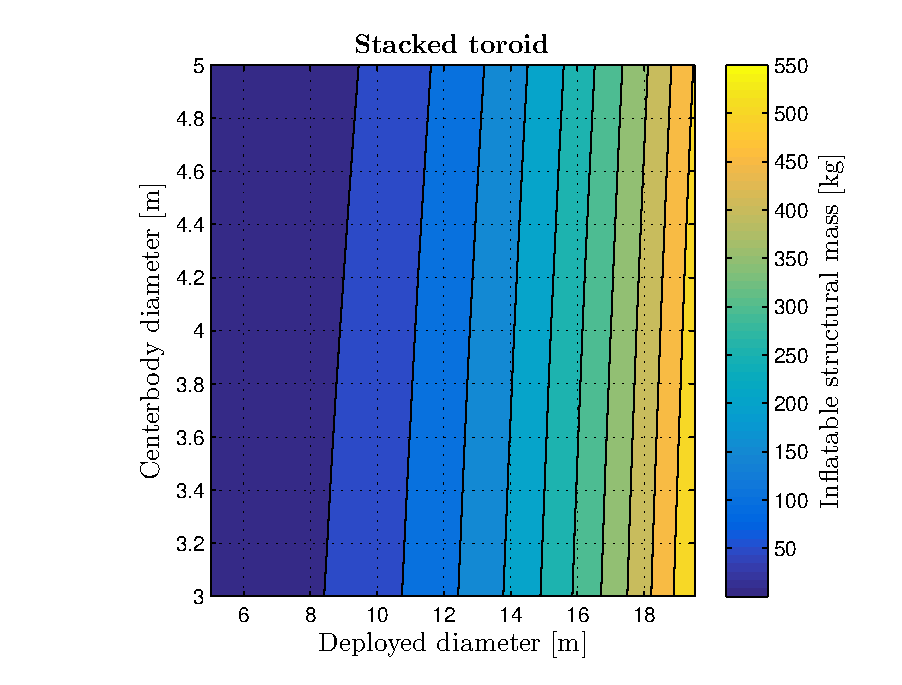
\includegraphics[width=0.96\textwidth]{./Figure/Structure/diameters_test.eps}
		\caption{Unrolling strut \cite[p.222]{Jenkins2001}}
		\label{fig:rot}
	\end{subfigure}
	\begin{subfigure}[b]{0.49\textwidth}
		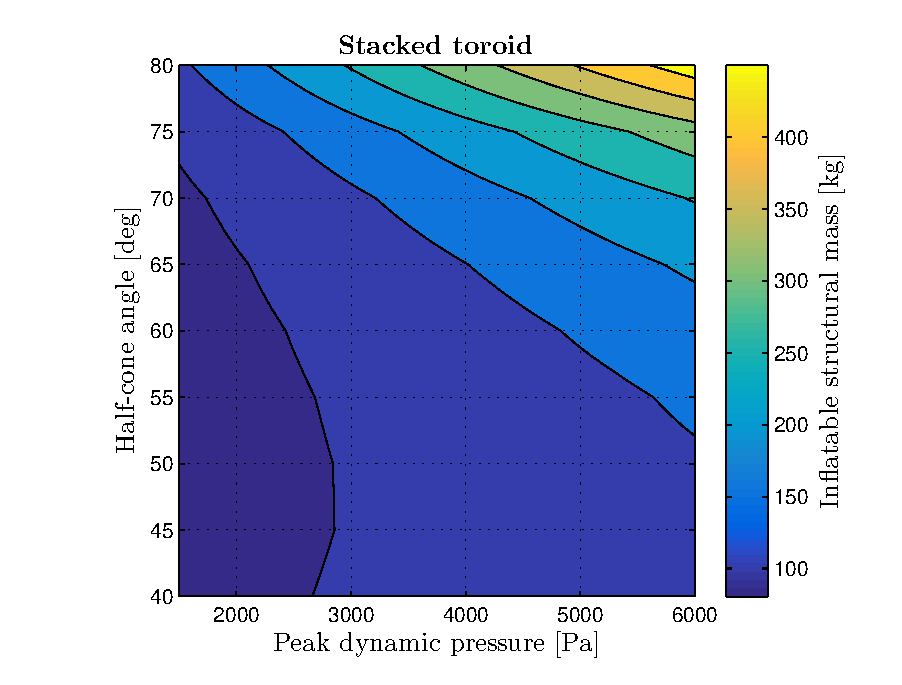
\includegraphics[width=0.96\textwidth]{./Figure/Structure/halfcone_test.eps}
		\caption{Unfolding strut \cite[p.226]{Jenkins2001}}
		\label{fig:fold}
	\end{subfigure}
	\begin{subfigure}[b]{0.49\textwidth}
		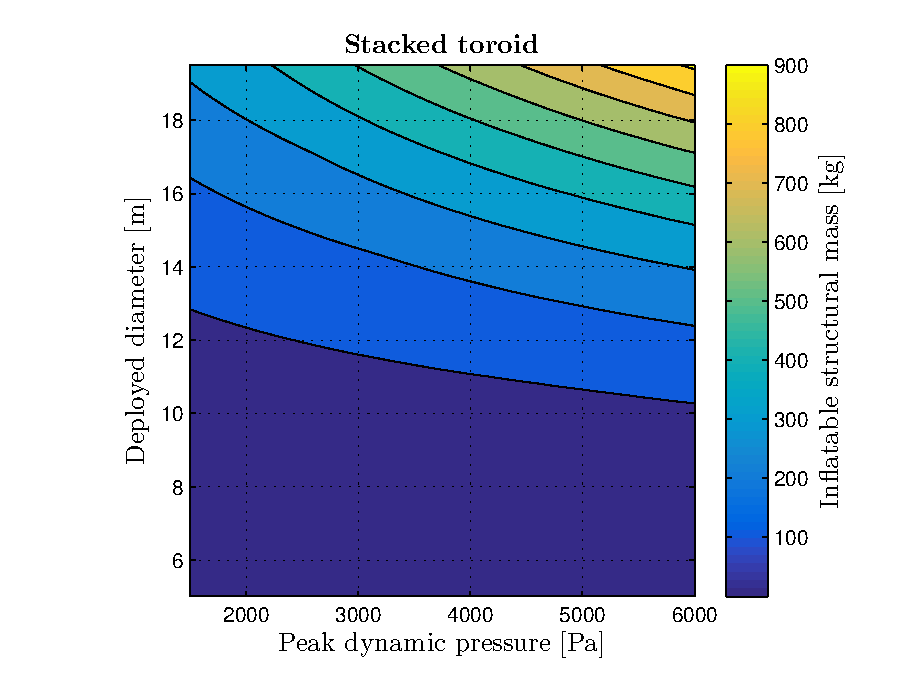
\includegraphics[width=0.96\textwidth]{./Figure/Structure/pressure_test.eps}
		\caption{Unrolling strut \cite[p.222]{Jenkins2001}}
		\label{fig:rot}
	\end{subfigure}
	\begin{subfigure}[b]{0.49\textwidth}
		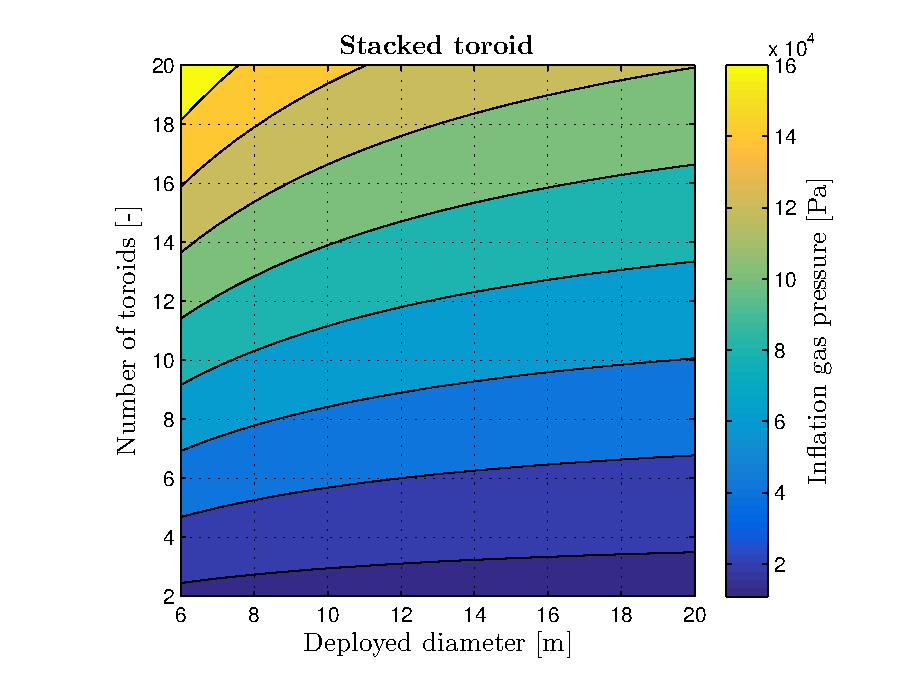
\includegraphics[width=0.96\textwidth]{./Figure/Structure/inflation_test.eps}
		\caption{Unfolding strut \cite[p.226]{Jenkins2001}}
		\label{fig:fold}
	\end{subfigure}
\end{figure}
Firstly, from Figure \ref{fig:diameters_strucmass} it follows that mass decreases with an increasing centerbody diameter given a deployed diameter. This is due to the fact that an increasing centerbody diameter increases the areal contribution of the centerbody: the inflatable requires less structural mass by decreased aerodynamic loading thereof, as aerodynamic pressure works over an area. In turn, this suggests that the centerbody becomes heavier, which is not the case as the centerbody is typically sized for launch rather than (re-)entry loads \cite{Lindell2006}. It can therefore be concluded that maximizing centerbody diameter is beneficial for structural mass. 

Secondly, from Figure \ref{fig:press_strucmass} it follows that increasing dynamic pressure effects an increase in structural mass of the inflatable. This is the result of an increased aerodynamic loading and therefore structural taxation of the inflatable. To withstand this loading, extra structural mass is required. Moreover, for a given peak dynamic pressure an increase in deployed diameter effects an increase in structural mass. Primary cause hereof is the fact that pressure works over a surface area and an increase in area thereby increases the loading. This is further amplified by an increase in bending moments by the larger distance from tip to root.

[MASS VERSUS DYN]

From Figure \ref{fig:halfcone_strucmass} it may be observed that the half-cone angle significantly affects inflatable structural mass: in general smaller half-cone angles are preferable. This is due to the fact that a smaller half-cone angle [XXX]

In Figure \ref{fig:inflpress_strucmass} Inflation gas pressure is observed to increase for an increasing number of toroids and to decrease with an increasing deployed diameter. Both an increase in the number of toroids and a decrease in deployed diameter decrease toroid radii, effecting an increase in the working area of the inflation pressure. Due to the proportionality of the running load induced by inflation pressure via Equation \ref{eq:inflationpressure} with toroid radius, a larger inflation pressure is required to induce the same running load with a smaller radius. This running load is based on the consideration that the work done by inflation gas and external forces in axial direction are equal \cite{Brown2009}, independent of the number of toroids. It is similarly independent of the deployed diameter, since both inflation and aerodynamic pressure have the same working area in axial direction.

[MATERIALS]

\begin{figure}[h]
	\centering

	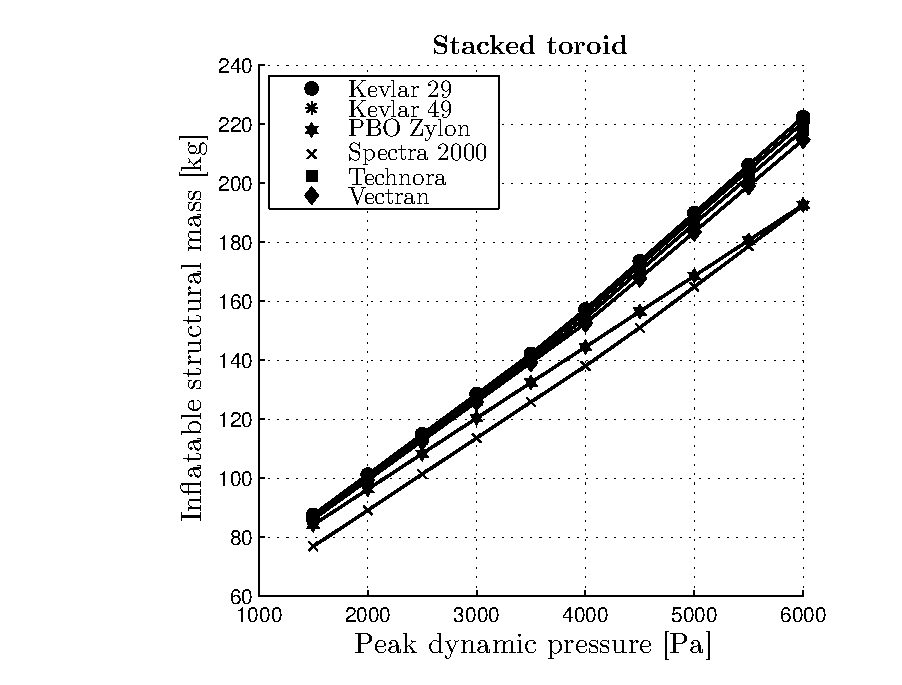
\includegraphics[width=0.6\textwidth]{./Figure/Structure/material_test.eps}
	\caption{Unrolling strut \cite[p.222]{Jenkins2001}}
	\label{fig:rot}
\end{figure}





